\documentclass[12pt]{article}

\usepackage[letterpaper,margin=1in]{geometry}

\setlength{\parindent}{0pt}

\usepackage{amssymb}
\usepackage{amsmath}

\usepackage{multicol}

\usepackage{tikz}

\newcommand{\headerText}{
  MA 126-103 | Summer 2017 | Dr. Clontz | 2017 July 24 Quiz
}

\usepackage{fancyhdr}
\pagestyle{fancy}
\renewcommand{\headrulewidth}{0pt}% Default \headrulewidth is 0.4pt
\renewcommand{\footrulewidth}{0pt}% Default \footrulewidth is 0pt
\chead{\footnotesize\bf\headerText}
\cfoot{}

\newcommand{\csch}{\operatorname{csch}}
\newcommand{\sech}{\operatorname{sech}}

\newcommand{\vect}{\mathbf}
\newcommand{\<}{\left\langle}
\renewcommand{\>}{\right\rangle}


\newcommand{\exerciseHeader}[4]{

  % \vspace{1em}
  %
  % \begin{tikzpicture}[x=1in,y=1in]
  %   \draw[color=black!50] (0,0) rectangle (6.4,1);
  %   \draw[color=black!50] (5.4,0) -- (5.4,1);
  %   \draw[dashed,color=black!20] (5.4,0.25) -- (6.4,0.25);
  %
  %   \node[anchor=north west,text width=4in,color=black!70] at (0,1) {\footnotesize Standard: This student is able to...};
  %   \node[anchor=north west,text width=4.5in] at (0.05,0.8) {\textbf{#2} #3};
  %   \node[anchor=south west,color=black!70] at (0, 0) {\footnotesize #4};
  %
  %   \node[anchor=north west,color=black!70] at (5.4,0.95) {\footnotesize Mark:};
  %   \node[anchor=south east,color=black!70] at (5.4,0) {\footnotesize \(\star\) reattempt due on:};
  % \end{tikzpicture}
  %
  % \vspace{1em}

  \vspace{0.5em}
  \textbf{#2}
  \vspace{0.5em}

}

\newcommand{\exerciseHeaderAnswer}[4]{

\newpage

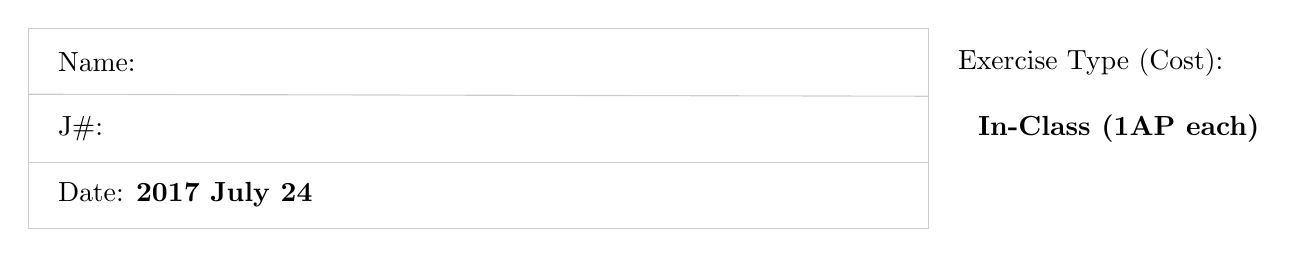
\begin{tikzpicture}[x=1in,y=1in]
  \draw[color=black!20] (0,0) rectangle (4.5,1);
  \draw[color=black!20] (0,0.67) -- (4.5,0.66);
  \draw[color=black!20] (0,0.33) -- (4.5,0.33);

  \node[anchor=west] at (0.1,0.83) {Name:};
  \node[anchor=west] at (0.1,0.5) {J\#:};
  \node[anchor=west] at (0.1,0.17) {Date: \textbf{2017 July 24}};

  \node[anchor=west] at (4.6,0.83) {Exercise Type (Cost):};
  \node[anchor=west] at (4.7,0.5) {\textbf{In-Class (1AP each)}};
\end{tikzpicture}

  \vspace{1em}

  \begin{tikzpicture}[x=1in,y=1in]
    \draw[color=black!50] (0,0) rectangle (6.4,1);
    \draw[color=black!50] (5.4,0) -- (5.4,1);
    \draw[dashed,color=black!20] (5.4,0.25) -- (6.4,0.25);

    \node[anchor=north west,text width=4in,color=black!70] at (0,1) {};
    \node[anchor=north west,text width=4.5in] at (0.05,0.8) {\textbf{#2} #3};
    \node[anchor=south west,color=black!70] at (0, 0) {\footnotesize #4};

    \node[anchor=north west,color=black!70] at (5.4,0.95) {\footnotesize Mark:};
    \node[anchor=south east,color=black!70] at (5.4,0) {\footnotesize \(\star\) reattempt due on:};
  \end{tikzpicture}

  \vspace{1em}

}



\begin{document}

\begin{multicols}{2}

% \exerciseHeader{2017 June 01}{C01: LogExpDerInt.}{
% Find derivatives and integrals involving logrithmic and exponential functions.
% }{1/4}
%
% a) Find \(\frac{d}{dx}[ex+\ln(2x)]\).
%
% \vfill
%
% b) Find \(\int(\frac{4}{x}-3e^x)\,dx\).
%
% \vfill

% \exerciseHeader{2017 June 02}{C01: LogExpDerInt.}{
% Find derivatives and integrals involving logrithmic and exponential functions.
% }{2/4}
%
% a) Find \(\frac{d}{dt}[5e^{2t}+\frac{1}{t}]\).
%
% \vfill
%
% b) Find \(\int\frac{z^3+2z+4}{z}\,dz\).
%
% \vfill

% \exerciseHeader{2017 June 06}{C01: LogExpDerInt.}{
% Find derivatives and integrals involving logrithmic and exponential functions.
% }{3/4}
%
% Prove that \(\int (2ye^{y^2}+\frac{4}{y})\,dy=e^{y^2}+4\ln|3y|+C\).

% \exerciseHeader{2017 June 07}{C01: LogExpDerInt.}{
% Find derivatives and integrals involving logrithmic and exponential functions.
% }{4/4}
%
% Prove that \(\int \frac{x^2e^x+4x}{x^2}dx=e^x+\ln(x^4)+C\).

\exerciseHeader{2017 June 07}{C01: LogExpDerInt.}{
Find derivatives and integrals involving logrithmic and exponential functions.
}{Extra}

Find \(\frac{d}{dx}[\ln(3e^x)]\).



% \exerciseHeader{2017 June 02}{S01: LogExpPrf.}{
% Derive properties of the logarithmic and exponential functions from their definitions.
% }{1/3}
%
% Prove that \(\ln(ax)=\ln(a)+\ln(x)\).

% \exerciseHeader{2017 June 06}{S01: LogExpPrf.}{
% Derive properties of the logarithmic and exponential functions from their definitions.
% }{2/3}
%
% Use the definitions
% \( \log_b x = \frac{\ln x}{\ln b} \) and \(b^x = \exp(x\ln b)\)
% to prove the property \( x = \log_b(b^x) \). (That is, prove that
% \(\log_b x\) and \(b^x\) are inverse functions.)

% \exerciseHeader{2017 June 07}{S01: LogExpPrf.}{
% Derive properties of the logarithmic and exponential functions from their definitions.
% }{3/3}
%
% Use \(\frac{d}{dx}[\ln(x)]=\frac{1}{x}\) and \(\ln(1)=0\) to
% prove that \(\ln(\frac{x^2}{4})=2\ln(x)-\ln(4)\).

\exerciseHeader{2017 June 07}{S01: LogExpPrf.}{
Derive properties of the logarithmic and exponential functions from their definitions.
}{3/3}

Use \(\frac{d}{dx}[\ln(x)]=\frac{1}{x}\), \(\ln(1)=0\), and \(\ln(e)=1\) to
prove that \(\ln(ex)=\ln(x)+1\).



% \exerciseHeader{2017 June 06}{C02: HypDerInt.}{
% Find derivatives and integrals involving hypberbolic functions.
% }{1/4}
%
% a) Find \(\frac{d}{dx}[\cosh(3x^2+7)]\).
%
% \vfill
%
% b) Find \(\int(5\sech^2(x)-4\csch(x)\coth(x))\,dx\).
%
% \vfill

% \exerciseHeader{2017 June 07}{C02: HypDerInt.}{
% Find derivatives and integrals involving hypberbolic functions.
% }{2/4}
%
% a) Find \(\frac{d}{dx}[\sinh(2x)-\tanh(x)]\).
%
% \vfill
%
% b) Find \(\int(\cosh(x^2)\sech(x^2))\,dx\).
%
% \vfill

% \exerciseHeader{2017 June 08}{C02: HypDerInt.}{
% Find derivatives and integrals involving hypberbolic functions.
% }{3/4}
%
% a) Find \(\frac{d}{dx}[e^x\cosh(x)]\).quiz-20170711
%
% \vfill
%
% b) Find \(\int(5\sinh(x)+\tanh(\pi))\,dx\).
%
% \vfill

% \exerciseHeader{2017 June 09}{C02: HypDerInt.}{
% Find derivatives and integrals involving hypberbolic functions.
% }{4/4}
%
% Show that \(\int4z\sech^2(z^2)\,dz=2\tanh(z^2)+C\).

\exerciseHeader{2017 June 09}{C02: HypDerInt.}{
Find derivatives and integrals involving hypberbolic functions.
}{4/4}

Find \(\frac{d}{dx}[x\cosh(3x)].\)


% \exerciseHeader{2017 June 07}{S02: HypPrf.}{
% Prove hyperbolic function identities.
% }{1/3}
%
% Use the definitions
% \[
%   \sinh(x)=\frac{e^x-e^{-x}}{2}
%     \hspace{3em}
%   \cosh(x)=\frac{e^x+e^{-x}}{2}
% \]
% to prove that \(\sinh^2(x)+\cosh^2(x)=\cosh(2x)\).
%
% \end{document}

% \exerciseHeader{2017 June 08}{S02: HypPrf.}{
% Prove hyperbolic function identities.
% }{2/3}
%
% Use the identity
% \[
%   \cosh^2(x)-\sinh^2(x)=1
% \]
% to prove the identity \(\coth^2(x)=1+\csch^2(x)\).

% \exerciseHeader{2017 June 09}{S02: HypPrf.}{
% Prove hyperbolic function identities.
% }{3/3}
%
% Use the definitions
% \[
%   \sinh(x)=\frac{e^x-e^{-x}}{2}
%     \hspace{3em}
%   \cosh(x)=\frac{e^x+e^{-x}}{2}
% \]
% to prove that \(\frac{d}{dx}[\sinh(x)]=\cosh(x)\).

\exerciseHeader{2017 June 09}{S02: HypPrf.}{
Prove hyperbolic function identities.
}{3/3}

Use the definitions
\[
  \sinh(x)=\frac{e^x-e^{-x}}{2}
    \hspace{3em}
  \cosh(x)=\frac{e^x+e^{-x}}{2}
\]
to prove that \(\frac{1}{2}\sinh(2x)=\sinh(x)\cosh(x)\).



% \exerciseHeader{2017 June 08}{C03: IntSub.}{
% Use integration by substitution.
% }{1/4}
%
% Find \(\int 120z(2z+1)^4\,dz\).

% \exerciseHeader{2017 June 09}{C03: IntSub.}{
% Use integration by substitution.
% }{2/4}
%
% Find \(\int \frac{z^2+1}{z^3+3z+7}\,dz\).

% \exerciseHeader{2017 June 13}{C03: IntSub.}{
% Use integration by substitution.
% }{3/4}
%
% Find \(\int 6x^2\sin(x^3)\,dx\).

% \exerciseHeader{2017 June 14}{C03: IntSub.}{
% Use integration by substitution.
% }{4/4}
%
% Recall that \(\int \frac{1}{1+x^2}\,du=\tan^\leftarrow(x)+C\).
% Find \(\displaystyle\int \frac{2e^y}{e^{2y}+1}\,dy\).

\exerciseHeader{2017 June 14}{C03: IntSub.}{
Use integration by substitution.
}{4/4}

Find \(\int x(x+4)^5\,dx\).



% \exerciseHeader{2017 June 09}{S03: TrigId.}{
% Integrate products of trigonometric functions by applying trigonometric
% identities.
% }{1/3}
%
% Find \(\int\sin^3\theta\cos^2\theta\,d\theta\).

% \exerciseHeader{2017 June 13}{S03: TrigId.}{
% Integrate products of trigonometric functions by applying trigonometric
% identities.
% }{2/3}
%
% Find \(\int\cos^2\theta\,d\theta\).

% \exerciseHeader{2017 June 14}{S03: TrigId.}{
% Integrate products of trigonometric functions by applying trigonometric
% identities.
% }{3/3}
%
% Find \(\int\tan^3\theta\sec^2\theta\,d\theta\).

\exerciseHeader{2017 June 14}{S03: TrigId.}{
Integrate products of trigonometric functions by applying trigonometric
identities.
}{3/3}

Find \(\int\cos^4(\theta)\sin^3(\theta)\,d\theta\).



% \exerciseHeader{2017 June 13}{S04: TrigSub.}{
% Use trigonometric substitution.
% }{1/3}
%
% Find \(\displaystyle\int\frac{4}{9+4y^2}\,dy\).

% \exerciseHeader{2017 June 14}{S04: TrigSub.}{
% Use trigonometric substitution.
% }{2/3}
%
% Recall that \(\sin(2\theta)=2\sin\theta\cos\theta\)
% and \(\cos^2(\theta)=\frac{1}{2}+\frac{1}{2}\cos(2\theta)\).
% Find \(\displaystyle\int\frac{2x^2}{\sqrt{4-x^2}}\,dx\).
%
% \exerciseHeader{2017 June 15}{S04: TrigSub.}{
% Use trigonometric substitution.
% }{3/3}
%
% Find \(\displaystyle\int\frac{x}{4-x^2}\,dx\) using the trigonometric substitution
% \(4-x^2=4-4\sin^2\theta\) and the integral
% \(\int\tan\theta\,d\theta=-\ln|\cos\theta|+C\).
%
\exerciseHeader{2017 June 15}{S04: TrigSub.}{
Use trigonometric substitution.
}{3/3}

Find \(\int\frac{1}{\sqrt{4-x^2}}\,dx\).


% \exerciseHeader{2017 June 14}{S05: PartFrac.}{
% Use partial fractions to integrate rational functions.
% }{1/3}
%
% Find \(\displaystyle\int\frac{2x+5}{x^2-x-2}\,dx\).

% \exerciseHeader{2017 June 15}{S05: PartFrac.}{
% Use partial fractions to integrate rational functions.
% }{2/3}
%
% Expand \(\displaystyle\frac{3x^2-2x+3}{(x^2+1)^2}\) using partial fractions.
% Do not integrate.

% \exerciseHeader{2017 June 16}{S05: PartFrac.}{
% Use partial fractions to integrate rational functions.
% }{3/3}
%
% Give the partial fraction expansion of
% \(\displaystyle\frac{f(x)}{x(x+1)^3(x^2+4)^2}\)
% in terms of the unknown constants \(A\) through \(H\), assuming
% \(f(x)\) is a polynomial of degree less than \(8\). Do not solve
% for \(A\) through \(H\).

\exerciseHeader{2017 June 15}{S05: PartFrac.}{
Use partial fractions to integrate rational functions.
}{2/3}

Expand \(\displaystyle\frac{x^2+2}{x^3+x}\) using partial fractions.
Do not integrate.



% \exerciseHeader{2017 June 15}{C04: IntParts.}{
% Use integration by parts.
% }{1/4}
%
% Find \(\int 3x^2e^x\,dx\).

% \exerciseHeader{2017 June 16}{C04: IntParts.}{
% Use integration by parts.
% }{2/4}
%
% Find \(\int 8\sin(x)\cosh(x)\,dx\). (Note that one factor is trigonometric sine,
% the other is hyperbolic cosine, so integration by parts is in fact necessary.)

% \exerciseHeader{2017 June 19}{C04: IntParts.}{
% Use integration by parts.
% }{3/4}
%
% Find \(\int x\sin(2x)\,dx\).

% \exerciseHeader{2017 June 20}{C04: IntParts.}{
% Use integration by parts.
% }{4/4}
%
% Find \(\int 3x^2\ln(x)\,dx\).

% \exerciseHeader{2017 July 05}{C04: IntParts.}{
% Use integration by parts.
% }{Extra1}
%
% Find \(\int x^2\cos(x)\,dx\).

% \exerciseHeader{2017 July 06}{C04: IntParts.}{
% Use integration by parts.
% }{Extra2}
%
% Find \(\int 2x^5\ln(x)\,dx\).

\exerciseHeader{2017 July 06}{C04: IntParts.}{
Use integration by parts.
}{Extra2}

Find \(\int 4x^2\sin(2x)\,dx\).



% \exerciseHeader{2017 June 16}{C05: IntTech. }{
% Identify appropriate integration techniques.
% }{1/4}
%
% Draw lines matching each of the five integrals on the left withquiz-20170711
%
% \begin{multicols}{2}
%   \begin{itemize}
%     \item[] \(\displaystyle\int x\sin(x)\,dx\)
%     \item[] \(\displaystyle\int \cos^4(x)\,dx\)
%     \item[] \(\displaystyle\int\frac{1}{x\sqrt{x^2+1}}\,dx\)
%     \item[] \(\displaystyle\int\frac{4x}{3x^2-1}\,dx\)
%     \item[] \(\displaystyle\int\frac{7x^2+x+12}{x^3+3x}\,dx\)
%   \end{itemize}
%   \columnbreak
%   \begin{itemize}
%     \item Integration by Substiution
%     \item Method of Partial Fractions
%     \item Trigonometric Identities
%     \item Trigonometric Substitution
%     \item Integration by Parts
%   \end{itemize}
% \end{multicols}
%
% \exerciseHeader{2017 June 19}{C05: IntTech. }{
% Identify appropriate integration techniques.
% }{2/4}
%
% Draw lines matching each of the five integrals on the left with
% the most appropriate integration technique listed on the right.
% Multiple techniques may be technically possible, but choose the technique most
% useful to begin integration. Every integral and technique is used exactly
% once in the correct answer.
%
% \vspace{1em}
%
% \begin{multicols}{2}
%   \begin{itemize}
%     \item[] \(\displaystyle\int\frac{x^3}{\sqrt{4-x^2}}\,dx\)
%     \item[] \(\displaystyle\int x^2\cos(x)\,dx\)
%     \item[] \(\displaystyle\int\cos^2(x)\,dx\)
%     \item[] \(\displaystyle\int\frac{x+4}{x^2+3x+2}\,dx\)
%     \item[] \(\displaystyle\int x\cos(x^2)\,dx\)
%   \end{itemize}
%   \columnbreak
%   \begin{itemize}
%     \item Integration by Substiution
%     \item Method of Partial Fractions
%     \item Trigonometric Identities
%     \item Trigonometric Substitution
%     \item Integration by Parts
%   \end{itemize}
% \end{multicols}

% \exerciseHeader{2017 June 20}{C05: IntTech. }{
% Identify appropriate integration techniques.
% }{3/4}
%
% Draw lines matching each of the five integrals on the left with
% the most appropriate integration technique listed on the right.
% Multiple techniques may be technically possible, but choose the technique most
% useful to begin integration. Every integral and technique is used exactly
% once in the correct answer.
%
% \vspace{1em}
%
% \begin{multicols}{2}
%   \begin{itemize}
%     \item[] \(\displaystyle\int\frac{x^2-4x+7}{(x^2+4)(x-2)}\,dx\)
%     \item[] \(\displaystyle\int\frac{16x^2}{\sqrt{4+x^2}}\,dx\)
%     \item[] \(\displaystyle\int x^3e^x\,dx\)
%     \item[] \(\displaystyle\int \frac{\sin(\ln(x))}{x}\,dx\)
%     \item[] \(\displaystyle\int\frac{1}{\cos^4(x)}\,dx\)
%   \end{itemize}
%   \columnbreak
%   \begin{itemize}
%     \item Integration by Substiution
%     \item Method of Partial Fractions
%     \item Trigonometric Identities
%     \item Trigonometric Substitution
%     \item Integration by Parts
%   \end{itemize}
% \end{multicols}

% \exerciseHeader{2017 June 21}{C05: IntTech. }{
% Identify appropriate integration techniques.
% }{4/4}
%
% Draw lines matching each of the five integrals on the left with
% the most appropriate integration technique listed on the right.
% Multiple techniques may be technically possible, but choose the technique most
% useful to begin integration. Every integral and technique is used exactly
% once in the correct answer.
%
% \vspace{1em}
%
% \begin{multicols}{2}
%   \begin{itemize}
%     \item[] \(\displaystyle\int\sin^4(x)\cos^3(x)\,dx\)
%     \item[] \(\displaystyle\int\frac{x^3+4x-1}{(x+4)(x^2+5)^2}\,dx\)
%     \item[] \(\displaystyle\int 6x^2\sqrt{1+x^3}\,dx\)
%     \item[] \(\displaystyle\int \sin(2x)e^x\,dx\)
%     \item[] \(\displaystyle\int\frac{4}{x^2\sqrt{x^2-1}}\,dx\) where \(x>1\)
%   \end{itemize}
%   \columnbreak
%   \begin{itemize}
%     \item Integration by Substiution
%     \item Method of Partial Fractions
%     \item Trigonometric Identities
%     \item Trigonometric Substitution
%     \item Integration by Parts
%   \end{itemize}
% \end{multicols}

\columnbreak

\exerciseHeader{2017 June 21}{C05: IntTech. }{
Identify appropriate integration techniques.
}{4/4}

Which integration technique is most appropriate for each integral?

  \begin{enumerate}
    \item \(\int\sin^4(x)\cos^3(x)\,dx\)
    \item \(\int\frac{x^3+4x-1}{(x+4)(x^2+5)^2}\,dx\)
    \item \(\int 6x^2\sqrt{1+x^3}\,dx\)
    \item \(\int \sin(2x)e^x\,dx\)
    \item \(\int\frac{4}{x^2\sqrt{x^2-1}}\,dx\) where \(x>1\)
  \end{enumerate}
  \begin{itemize}\footnotesize
    \item Integration by Substiution
    \item Method of Partial Fractions
    \item Trigonometric Identities
    \item Trigonometric Substitution
    \item Integration by Parts
  \end{itemize}



% \exerciseHeader{2017 June 19}{C06: AreaBtCurv. }{
% Express an area between curves as a definite integral.
% }{1/4}
%
% Find a definite integral equal to the area bounded by
% \(y=2x^2+x\) and \(y=x^2-x+3\).

% \exerciseHeader{2017 June 20}{C06: AreaBtCurv. }{
% Express an area between curves as a definite integral.
% }{2/4}
%
% Find a definite integral equal to the area bounded by
% \(y=x^3\) and \(y=x\).

% \exerciseHeader{2017 June 21}{C06: AreaBtCurv. }{
% Express an area between curves as a definite integral.
% }{3/4}
%
% Find a definite integral equal to the area bounded by
% \(y=x\), \(y=2x-1\), and \(x=2\).

% \exerciseHeader{2017 June 22}{C06: AreaBtCurv. }{
% Express an area between curves as a definite integral.
% }{4/4}
%
% Find a definite integral equal to the area bounded by
% \(y=x\), \(y=2x-1\), and \(x=2\).

% \exerciseHeader{2017 July 13}{C06: AreaBtCurv. }{
% Express an area between curves as a definite integral.
% }{Extra1}
%
% Find a definite integral equal to the area bounded by
% \(y=2x\) and \(y=2x^2-4x\).

% \exerciseHeader{2017 July 14}{C06: AreaBtCurv. }{
% Express an area between curves as a definite integral.
% }{Extra2}
%
% Find a definite integral equal to the area bounded by
% \(x=y^2+1\) and \(x=3-y^2\).

\exerciseHeader{2017 July 14}{C06: AreaBtCurv. }{
Express an area between curves as a definite integral.
}{Extra2}

Find a definite integral equal to the area bounded by
\(y=4-x^2\) and \(y=x^2+4\).



% \exerciseHeader{2017 June 21}{S06: CrossSect.}{
% Express an area between curves as a definite integral.
% }{1/3}
%
% Find a definite integral equal to the volume of the wedge-shaped
% solid whose base lays on the region \(0\leq x\leq 4\) and \(0\leq y\leq 2\),
% and whose cross-sections at each \(x\)-value are rectangles of height \(x\).

% \exerciseHeader{2017 June 22}{S06: CrossSect.}{
% Express an area between curves as a definite integral.
% }{2/3}
%
% Find a definite integral equal to the volume of a pyramid
% with height \(5\) units and a \(10\times15\) rectangular base.

% \exerciseHeader{2017 June 23}{S06: CrossSect.}{
% Express an area between curves as a definite integral.
% }{3/3}
%
% Find a definite integral equal to the volume of a solid with its base
% on the region \(0\leq y\leq\sqrt{9-x^2}\) and with trianglular
% cross-sections at each \(x\)-value with height \(4x\). (Do not solve this
% integral.)

\exerciseHeader{2017 June 23}{S06: CrossSect.}{
Express an area between curves as a definite integral.
}{3/3}

Find a definite integral equal to the volume of a pyramid of height
\(6\) that has a square base of side length \(3\).



% \exerciseHeader{2017 June 23}{C07: WashShell.}{
% Use the washer or cylindrical shell method to express a volume of
% revolution as a definite integral.
% }{1/4}
%
% Find a definite integral equal to the volume of the solid obtained by
% rotating the region bounded by \(y=x^2\), \(y=0\), and \(x=2\) around
% the \(y\)-axis.

% \exerciseHeader{2017 June 26}{C07: WashShell.}{
% Use the washer or cylindrical shell method to express a volume of
% revolution as a definite integral.
% }{2/4}
%
% Find a definite integral equal to the volume of the solid obtained by
% rotating the region bounded by \(y=x^2-2x+1\) and \(y=x-1\) around
% the axis \(x=1\).

% \exerciseHeader{2017 June 27}{C07: WashShell.}{
% Use the washer or cylindrical shell method to express a volume of
% revolution as a definite integral.
% }{3/4}
%
% Find a definite integral equal to the volume of the solid obtained by
% rotating the triangle with vertices \((1,4),(1,2),(3,2)\) around
% the \(x\)-axis.
%
% \exerciseHeader{2017 June 28}{C07: WashShell.}{
% Use the washer or cylindrical shell method to express a volume of
% revolution as a definite integral.
% }{4/4}
%
% Find a definite integral equal to the volume of the solid obtained by
% rotating the region bounded by \(y=x\), \(y=2x\), \(y=2\) around
% the \(y\)-axis.

% \exerciseHeader{2017 July 05}{C07: WashShell.}{
% Use the washer or cylindrical shell method to express a volume of
% revolution as a definite integral.
% }{Extra1}
%
% Find a definite integral equal to the volume of the solid obtained by
% rotating the region bounded by \(y=\sqrt{x}\) and \(y=x\) around
% the \(y\)-axis.
%
% \exerciseHeader{2017 July 07}{C07: WashShell.}{
% Use the washer or cylindrical shell method to express a volume of
% revolution as a definite integral.
% }{Extra2}
%
% Find a definite integral equal to the volume of the solid obtained by
% rotating the region bounded by \(y=x\), \(y=2x\), \(x=3\) around
% the axis \(x=-1\).
%
\exerciseHeader{2017 July 07}{C07: WashShell.}{
Use the washer or cylindrical shell method to express a volume of
revolution as a definite integral.
}{Extra2}

Find a definite integral equal to the volume of the solid obtained by
rotating the region bounded by \(y=x\), \(y=2x\), \(y=4\) around
the axis \(y=-1\).



% \exerciseHeader{2017 June 26}{C08: Work.}{
% Express the work done in a system as a definite integral.
% }{1/4}
%
% Find a definite integral equal to the work required to pull up \(25\) meters
% of cable if it weighs \(100\) newtons and is fully extended downward into
% a hole.

% \exerciseHeader{2017 June 27}{C08: Work.}{
% Express the work done in a system as a definite integral.
% }{2/4}
%
% Hooke's Law states that the force required to stretch or
% compress a spring \(x\) units
% from its natural length requires \(F(x)=kx\) units of force for some
% constant \(k\) (depending on the spring). Suppose a spring satisfies
% \(k=7\) and is naturally length \(10\). Find a definite integral equal
% to the work required to compress
% this spring from length \(8\) to length \(5\).
% (Do not solve your integral.)

% \exerciseHeader{2017 June 28}{C08: Work.}{
% Express the work done in a system as a definite integral.
% }{3/4}
%
% As a worker lifted a leaky sandbag from the ground, it lost sand weight at
% a constant rate. Assuming it weighed \(20\) pounds on the ground, and
% weighed \(14\) pounds after being lifted \(2\) feet, what work was
% required to lift the sandbag \(2\) feet?
% (Do not solve your integral.)

% \exerciseHeader{2017 June 29}{C08: Work.}{
% Express the work done in a system as a definite integral.
% }{4/4}
%
% A \(100\) pound wrecking ball hanging from a \(20\) foot, \(40\) pound
% cable was hoisted up from a crane. Give a definite integral equal to the
% work required to pull up the ball and cable.
% (Do not solve your integral.)

% \exerciseHeader{2017 July 10}{C08: Work.}{
% Express the work done in a system as a definite integral.
% }{Extra1}
%
% As a worker lifted a leaky sandbag from the ground, it lost sand weight at
% a constant rate. Assuming it weighed \(30\) newtons on the ground, and
% weighed \(15\) newtons after being lifted \(3\) meters, what work was
% required to lift the sandbag \(3\) meters?
% (Do not solve your integral.)

% \exerciseHeader{2017 July 11}{C08: Work.}{
% Express the work done in a system as a definite integral.
% }{Extra2}
%
% Hooke's Law states that the force required to stretch or
% compress a spring \(x\) units
% from its natural length requires \(F(x)=kx\) units of force for some
% constant \(k\) (depending on the spring). Suppose a spring satisfies
% \(k=3\) and is naturally length \(5\). Find a definite integral equal
% to the work required to compress
% this spring from length \(4\) to length \(2\).
% (Do not solve your integral.)



% \exerciseHeader{2017 June 26}{S07: WorkDiff.}{
% Use the work differential to express the work done in pumping a tank of
% liquid as a definite integral.
% }{1/3}
%
% Assume salt water weighs \(10kN/m^3\).
% Find an expression in terms of \(y\) for the work differential \(dW\)
% required to pump a cross-section of water at height \(y\)
% from a pyramid-shaped tank with its tip pointing downwards, with a
% total height of \(4\) feet,
% and with a square lid with side length \(8\) feet. Then give a definite
% integral equal to the work required to pump this tank if it filled
% \(3\) feet deep with salt water.

% \exerciseHeader{2017 June 27}{S07: WorkDiff.}{
% Use the work differential to express the work done in pumping a tank of
% liquid as a definite integral.
% }{2/3}
%
% Assume salt water weighs \(10kN/m^3\).
% Find an expression in terms of \(y\) for the work differential \(dW\)
% required to pump a cross-section of water at height \(y\)
% from a cubical tank with side length \(5\) meters laying flat on the ground
% to its top.
% Then give a definite
% integral equal to the work required to pump this tank if it filled
% % \(4\) meters deep with salt water.
%
% \exerciseHeader{2017 June 28}{S07: WorkDiff.}{
% Use the work differential to express the work done in pumping a tank of
% liquid as a definite integral.
% }{3/3}
%
% Assume salt water weighs \(10kN/m^3\).
% Find an expression in terms of \(y
% Then give a definite
% integral equal to the work required to pump this tank if it was
% completely filled with salt water.
% (Do not solve your integral.)

\exerciseHeader{2017 June 27}{S07: WorkDiff.}{
Use the work differential to express the work done in pumping a tank of
liquid as a definite integral.
}{2/3}

Assume salt water weighs \(10kN/m^3\).
Find an expression in terms of \(y\) for the work differential \(dW\)
required to pump a cross-section of water at height \(y\)
from a rectangular tank that stands \(4\) meters tall, with a
\(3\times 5\) meter base.
Then give a definite
integral equal to the work required to pump this tank if it filled
\(2\) meters deep with salt water.



% \exerciseHeader{2017 June 28}{C09: Param.}{
% Parametrize planar curves and sketch parametrized curves.
% }{1/4}
%
% Parametrize the curve \(x^2+(y-4)^2=9\) starting at the point
% \((7,0)\) and rotating around the circle exactly once counter-clockwise.

% \exerciseHeader{2017 June 29}{C09: Param.}{
% Parametrize planar curves and sketch parametrized curves.
% }{2/4}
%
% Parametrize the line segment beginning at the point \((3,-4)\) and ending
% at the point \((-1,-1)\).

% \exerciseHeader{2017 June 30}{C09: Param.}{
% Parametrize planar curves and sketch parametrized curves.
% }{3/4}
%
% Parametrize the curve \(x=y^2\) from \((4,2)\) to \((9,3)\).

% \exerciseHeader{2017 July 05}{C09: Param.}{
% Parametrize planar curves and sketch parametrized curves.
% }{4/4}
%
% Consider the circle of radius \(3\) and center \((1,1)\).
% Parametrize the clockwise-oriented circular arc starting at \((1,4)\)
% and ending at \((4,1)\).



% \exerciseHeader{2017 June 29}{S08: ParamAppl.}{
% Parametrize a curve to find arclengths, surface areas, and slopes.
% }{1/3}
%
% The arclength of a curve parametrized by \(x,y\) in terms of \(t\)
% from \(a\leq t\leq b\) is given by
% \(\int_a^b\sqrt{(\frac{dx}{dt})^2+(\frac{dy}{dt})^2}\,dt\).
% Give a definite integral equal to the length of the arc along the
% curve \(y=x^3\) from \((-1,-1)\) to \((2,8)\).

% \exerciseHeader{2017 June 30}{S08: ParamAppl.}{
% Parametrize a curve to find arclengths, surface areas, and slopes.
% }{2/3}
%
% Consider the curve defined by the parametric equations
% \(x=4+4t^3\), \(y=t^2+2t+3\), \(0\leq t\leq 3\).
% Use the Chain Rule \(\frac{dy}{dt}=\frac{dy}{dx}\frac{dx}{dt}\) to
% find the point on the curve that has slope \(1/3\).

% \exerciseHeader{2017 July 05}{S08: ParamAppl.}{
% Parametrize a curve to find arclengths, surface areas, and slopes.
% }{3/3}
%
% The surface area obtained by rotating the curve parametrized by
% \(x(t)\) and \(y(t)\geq 0\) where \(a\leq t\leq b\) around the \(x\)-axis
% is given by \(2\pi\int_a^b y(t)\sqrt{(\frac{dx}{dt})^2+(\frac{dy}{dt})^2}\,dt\).
% Give a definite integral equal to the conical surface area obtained by
% rotating the line segment connecting \((1,0)\) and \((6,2)\) around the
% \(x\)-axis.



% \exerciseHeader{2017 June 30}{C10: Polar.}{
% Convert and sketch polar and Cartesian coordinates and equations.
% }{1/4}
%
% Find a polar equation for the line segment connecting \((3,0)\) and
% \((3,3)\).

% \exerciseHeader{2017 July 05}{C10: Polar.}{
% Convert and sketch polar and Cartesian coordinates and equations.
% }{2/4}
%
% Convert the Cartesian coordinates \((3,-3\sqrt 3)\) to polar.

% \exerciseHeader{2017 July 06}{C10: Polar.}{
% Convert and sketch polar and Cartesian coordinates and equations.
% }{3/4}
%
% Find a Cartesian equation for the circle defined by the polar equation
% \(r=6\sin\theta\). (Hint: Multiply both sides by \(r\), convert to
% \(x\) and \(y\), move all terms to the same side, add \(9\) to both sides
% of the equation, and then factor the \(y\) terms.)
% Then sketch the circle.

% \exerciseHeader{2017 July 07}{C10: Polar.}{
% Convert and sketch polar and Cartesian coordinates and equations.
% }{4/4}
%
% Draw the circle centered at the origin with radius \(2\), along with the
% line segments from \((0,0)\) to \((0,2)\) and from \((0,0)\) to
% \((\sqrt 2,\sqrt 2)\). Then describe the smaller region bounded by the circle
% and between these line segments using polar coordinates.

% \exerciseHeader{2017 July 18}{C10: Polar.}{
% Convert and sketch polar and Cartesian coordinates and equations.
% }{Extra1}
%
% Sketch the circle defined by \(x^2+(y-3)^2=9\). Then find a simplified
% polar equation that describes the same circle.

% \exerciseHeader{2017 July 19}{C10: Polar.}{
% Convert and sketch polar and Cartesian coordinates and equations.
% }{Extra2}
%
% Give an inequality involving polar coordinates that describes the
% fourth quadrant of the \(xy\) plane (where \(x\) is positive and
% \(y\) is negative).



% \exerciseHeader{2017 July 05}{S09: PolarAppl.}{
% Use polar coordinates to express an arclength or area as a definite integral.
% }{1/4}
%
% The area bounded by an outside curve with polar equation \(r=R(\theta)\)
% and inside curve with polar equation \(r=r(\theta)\) where
% \(\alpha\leq\theta\leq\beta\) is given by
% \(\frac{1}{2}\int_\alpha^\beta((R(\theta))^2-(r(\theta))^2)\,d\theta\).
% Give a definite integral equal to the area inside the cardioid
% \(r=2+2\cos\theta\) but outside the circle \(r=2\).

% \exerciseHeader{2017 July 06}{S09: PolarAppl.}{
% Use polar coordinates to express an arclength or area as a definite integral.
% }{2/3}
%
% The arclength of the curve defined by the polar equation \(r=r(\theta)\)
% where \(\alpha\leq\theta\leq\beta\) is given by
% \(\int_\alpha^\beta\sqrt{(r(\theta))^2+(\frac{dr}{d\theta})^2}\,d\theta\).
% Give a definite integral equal to the circumference of the cardioid
% \(r=3-3\sin\theta\).

% \exerciseHeader{2017 July 07}{S09: PolarAppl.}{
% Use polar coordinates to express an arclength or area as a definite integral.
% }{3/3}
%
% The area bounded by an outside curve with polar equation \(r=R(\theta)\)
% and inside curve with polar equation \(r=r(\theta)\) where
% \(\alpha\leq\theta\leq\beta\) is given by
% \(\frac{1}{2}\int_\alpha^\beta((R(\theta))^2-(r(\theta))^2)\,d\theta\).
% Give a definite integral equal to the area inside the circle
% \(x^2+y^2=2\) and to the left of the line \(x=-1\).



% \exerciseHeader{2017 July 06}{S10: SeqForm.}{
% Define and use explicit and recursive formulas for sequences.
% }{1/3}
%
% Complete the following proof by induction that the sequence
% \(\<3n^2+1\>_{n=1}^\infty\) may be defined
% recursively by \(a_1=4\) and \(a_{n+1}=a_n+6n+3\).
%
% We first verify that the explicit formula \(a_n=3n^2+1\) satisfies
% the base case \(a_1=4\):
%
% \vfill
%
% Now, assuming that \(a_n=3n^2+1\) holds for \(n\), we may use the recursive
% formula \(a_{n+1}=a_n+6n+3\) to show that \(a_{n+1}=3(n+1)^2+1\):
%
% \vfill\vfill

% \exerciseHeader{2017 July 07}{S10: SeqForm.}{
% Define and use explicit and recursive formulas for sequences.
% }{2/3}
%
% Find an explicit formula \(a_n\) for the sequence
% \(\<1,\frac{3}{2},\frac{5}{4},\frac{7}{8},\frac{9}{16},\frac{11}{32},\dots\>\).
% Then write the sequence in \(\<a_n\>_{n=N}^\infty\) form (where \(N\) is your
% starting index).

% \exerciseHeader{2017 July 11}{S10: SeqForm.}{
% Define and use explicit and recursive formulas for sequences.
% }{3/3}
%
% Find a recursive formula for the sequence \(\<3,4,6,9,13,18,\dots\>\).
% (You may choose whatever starting index you like.)



% \exerciseHeader{2017 July 07}{C11: SeqLim.}{
% Compute the limit of a convergent sequence.
% }{1/4}
%
% Use factoring to find
% \(\displaystyle\lim_{k\to\infty}\frac{k^3-2k^2+7}{1+k^4}\).

% \exerciseHeader{2017 July 11}{C11: SeqLim.}{
% Compute the limit of a convergent sequence.
% }{2/4}
%
% Use L'Hoptial's Rule to find
% \(\displaystyle\lim_{m\to\infty}\frac{e^{m^2}+7}{e^{m^2+1}}\).

% \exerciseHeader{2017 July 12}{C11: SeqLim.}{
% Compute the limit of a convergent sequence.
% }{3/4}
%
% Recall that the recursive defintion of a factorial is given by
% \(0!=1\) and \((n+1)!=n!(n+1)\). Find
% \(\displaystyle\lim_{n\to\infty}\frac{\frac{3^{n+1}}{(n+1)!}}{\frac{3^n}{n!}}\).

% \exerciseHeader{2017 July 13}{C11: SeqLim.}{
% Compute the limit of a convergent sequence.
% }{4/4}
%
% Find \(\displaystyle\lim_{m\to\infty}\frac{3-m^2}{4m^2-5m+7}\).


% \exerciseHeader{2017 July 11}{C12: PartSum.}{
% Find the value of a convergent series by expressing it as a limit of
% partial sums.
% }{1/4}
%
% Find a formula for the partial sum \(s_n=a_0+a_1+\dots+a_n\) where
% \(a_n=\frac{2}{3^n}\). Then use this formula to prove that
% \(\sum_{m=0}^\infty\frac{2}{3^m}=2+\frac{2}{3}+\frac{2}{9}+\dots=3\).

% \exerciseHeader{2017 July 12}{C12: PartSum.}{
% Find the value of a convergent series by expressing it as a limit of
% partial sums.
% }{2/4}
%
% Find a formula for the partial sum \(s_n=a_0+a_1+\dots+a_n\) where
% \(a_n=(\frac{3n+4}{n+1}-\frac{3n+7}{n+2})\). Then use this formula to prove that
% \(\sum_{n=0}^\infty(\frac{3n+4}{n+1}-\frac{3n+7}{n+2})=1\).

% \exerciseHeader{2017 July 13}{C12: PartSum.}{
% Find the value of a convergent series by expressing it as a limit of
% partial sums.
% }{3/4}
%
% Recall that \(\lim_{n\to\infty}x^n\) diverges when \(|x|\geq 1\).
% Find a formula for the partial sum \(s_n=a_0+a_1+\dots+a_n\) where
% \(a_n=\frac{2^{2n}}{3^n}\). Then use this formula to prove that
% \(\sum_{n=0}^\infty \frac{2^{2n}}{3^n}\) diverges.

% \exerciseHeader{2017 July 14}{C12: PartSum.}{
% Find the value of a convergent series by expressing it as a limit of
% partial sums.
% }{4/4}
%
% Find a formula for the partial sum \(s_n=a_0+a_1+\dots+a_n\) where
% \(a_n=(\frac{2}{n+3}-\frac{2}{n+4})\). Then use this formula to find the value
% of \(\sum_{n=0}^\infty (\frac{2}{n+3}-\frac{2}{n+4})=(\frac{2}{3}-\frac{2}{4})+
% (\frac{2}{4}-\frac{2}{5})+\dots\).



% \exerciseHeader{2017 July 12}{S11: GeoAlt.}{
% Determine if a geometric series or alternating series is convergent or
% divergent.
% }{1/3}
%
% Recall that the geometric series \(\sum_{n=0}^\infty ar^n\) converges to
% \(\frac{a}{1-r}\) when \(|r|<1\) and diverges otherwise.
%
% Does the series
% \(\sum_{k=1}^\infty 3^{-k}=\frac{1}{3}+\frac{1}{9}+\frac{1}{27}+\dots\)
% converge or diverge? If it converges, what it is value?

% \exerciseHeader{2017 July 13}{S11: GeoAlt.}{
% Determine if a geometric series or alternating series is convergent or
% divergent.
% }{2/3}
%
% Let \(a_n\) be positive and monotonic (non-increasing or non-decreasing).
% Recall that the alternating series \(\sum_{n=N}^\infty (-1)^n a_n\) converges
% if and only if \(\lim_{n\to\infty}a_n=0\).
%
% Does the series
% \(\sum_{k=2}^\infty (-1)^k\frac{k}{k^2+1}=\frac{2}{5}-\frac{3}{10}+
% \frac{4}{17}-\frac{5}{26}+\dots\)
% converge or diverge?

% \exerciseHeader{2017 July 14}{S11: GeoAlt.}{
% Determine if a geometric series or alternating series is convergent or
% divergent.
% }{3/3}
%
% Recall that the geometric series \(\sum_{n=0}^\infty ar^n\) converges to
% \(\frac{a}{1-r}\) when \(|r|<1\) and diverges otherwise.
%
% Does the series
% \(\sum_{k=1}^\infty(-1)^{k+1}\frac{5}{4^{k-1}}=
% 5-\frac{5}{4}+\frac{5}{16}-\frac{5}{64}+\dots\)
% converge or diverge? If it converges, what it is value?



% \exerciseHeader{2017 July 13}{S12: IntTest.}{
% Use the integral test to determine series convergence.
% }{1/3}
%
% Does \(\int_8^\infty\frac{3}{\sqrt[3]{x}}\,dx\) converge or diverge?
%
% \vfill\vfill
%
% Does \(\sum_{k=3}^\infty\frac{3}{\sqrt[3]{k}}\) converge or diverge?
%
% \vfill

% \exerciseHeader{2017 July 14}{S12: IntTest.}{
% Use the integral test to determine series convergence.
% }{2/3}
%
% Does \(\int_1^\infty\frac{2x}{x^2+1}\,dx\) converge or diverge?
%
% \vfill\vfill
%
% Does \(\sum_{m=0}^\infty\frac{2m}{m^2+1}\) converge or diverge?
%
% \vfill

% \exerciseHeader{2017 July 18}{S12: IntTest.}{
% Use the integral test to determine series convergence.
% }{3/3}
%
% Does \(\int_{11}^\infty\frac{1}{x(\ln x)^2}\,dx\) converge or diverge?
%
% \vfill\vfill
%
% Does \(\sum_{k=4}^\infty\frac{1}{k(\ln k)^2}\) converge or diverge?
%
% \vfill



% \exerciseHeader{2017 July 14}{S13: RatioRoot.}{
% Use the ratio and root tests to determine series convergence.
% }{1/3}
%
% Does \(\displaystyle\sum_{m=0}^\infty\frac{m!}{3^{2m}}=
% 1+\frac{1}{9}+\frac{2}{81}+\frac{6}{729}+\dots\) converge or diverge?

% \exerciseHeader{2017 July 18}{S13: RatioRoot.}{
% Use the ratio and root tests to determine series convergence.
% }{2/3}
%
% Recall that \(e^x=\lim_{n\to\infty}(1+x/n)^n\).
% Does \(\displaystyle\sum_{k=3}^\infty\left(1-\frac{2}{k}\right)^{2k^2}
% =(1/3)^{18}+(1/2)^{32}+(3/5)^{50}+\dots\)
% converge or diverge?

% \exerciseHeader{2017 July 19}{S13: RatioRoot.}{
% Use the ratio and root tests to determine series convergence.
% }{3/3}
%
% Use either the Ratio or Root Test to determine whether \(\displaystyle\sum_{n=0}^\infty\frac{4^n}{3^{2n+1}}
% =\frac{1}{3}+\frac{4}{27}+\frac{16}{243}+\dots\)
% converges or diverges.



% \exerciseHeader{2017 July 18}{S14: CompTests.}{
% Use the comparison tests to determine series convergence.
% }{1/3}
%
% Does \(\displaystyle\sum_{n=0}^\infty\frac{2^n}{4^n+\sqrt{n}}=
% 1+\frac{2}{5}+\frac{4}{16+\sqrt 2}+\dots\) converge or diverge?

% \exerciseHeader{2017 July 19}{S14: CompTests.}{
% Use the comparison tests to determine series convergence.
% }{2/3}
%
% Does \(\displaystyle\sum_{m=0}^\infty\frac{1}{\sqrt[3]{m^2+1}}=
% 1+\frac{1}{\sqrt[3]{2}}+\frac{1}{\sqrt[3]{5}}+\dots\) converge or diverge?

% \exerciseHeader{2017 July 20}{S14: CompTests.}{
% Use the comparison tests to determine series convergence.
% }{3/3}
%
% Does \(\displaystyle\sum_{n=2}^\infty\frac{5n}{n^3-1}=
% \frac{10}{7}+\frac{15}{26}+\frac{20}{63}+\dots\) converge or diverge?



% \exerciseHeader{2017 July 19}{C13: SerTech.}{
% Identify series as convergent or divergent along with appropriate techniques to
% determine convergence or divergence.
% }{1/4}
%
% For each series, choose \textbf{one} technique that
% would be appropriate to determine convergence/divergence. (There may be
% multiple correct responses.) Then choose
% whether the series is convergent or divergent. You do not need to show your
% work.
%
% \begin{multicols}{3}
% \(\sum_{k=1}^\infty\frac{k}{4+k^2}\)
%
% \vspace{1em}
%
% \begin{itemize}\footnotesize
% \item Partial Sum Sequence
% \item Divergence Test
% \item Geometric Series Test
% \item Alternating Series Test
% \item Integral Test
% \item p-Series Test
% \item Ratio Test
% \item Root Test
% \item Direct/Limit Comp. Test
% \end{itemize}
%
% \vspace{1em}
%
% \begin{itemize}\footnotesize
% \item Converges
% \item Diverges
% \end{itemize}
%
% \columnbreak
%
% \(\sum_{m=0}^\infty\frac{8^m}{3^{m+1}}\)
%
% \vspace{1em}
%
% \begin{itemize}\footnotesize
% \item Partial Sum Sequence
% \item Divergence Test
% \item Geometric Series Test
% \item Alternating Series Test
% \item Integral Test
% \item p-Series Test
% \item Ratio Test
% \item Root Test
% \item Direct/Limit Comp. Test
% \end{itemize}
%
% \vspace{1em}
%
% \begin{itemize}\footnotesize
% \item Converges
% \item Diverges
% \end{itemize}
%
% \columnbreak
%
% \(\sum_{n=2}^\infty(-1)^n\frac{1}{n^2}\)
%
% \vspace{1em}
%
% \begin{itemize}\footnotesize
% \item Partial Sum Sequence
% \item Divergence Test
% \item Geometric Series Test
% \item Alternating Series Test
% \item Integral Test
% \item p-Series Test
% \item Ratio Test
% \item Root Test
% \item Direct/Limit Comp. Test
% \end{itemize}
%
% \vspace{1em}
%
% \begin{itemize}\footnotesize
% \item Converges
% \item Diverges
% \end{itemize}
% \end{multicols}


% \exerciseHeader{2017 July 20}{C13: SerTech.}{
% Identify series as convergent or divergent along with appropriate techniques to
% determine convergence or divergence.
% }{2/4}
%2(-\frac{6}{5})^n
% For each series, choose \textbf{one} technique that
% would be appropriate to determine convergence/divergence. (There may be
% multiple correct responses.) Then choose
% whether the series is convergent or divergent. You do not need to show your
% work.
%
% \begin{multicols}{3}
% \(\sum_{k=1}^\infty\frac{3^k}{(k+1)5^k}\)
%
% \vspace{1em}
%
% \begin{itemize}\footnotesize
% \item Partial Sum Sequence
% \item Divergence Test
% \item Geometric Series Test
% \item Alternating Series Test
% \item Integral Test
% \item p-Series Test
% \item Ratio Test
% \item Root Test
% \item Direct/Limit Comp. Test
% \end{itemize}
%
% \vspace{1em}
%
% \begin{itemize}\footnotesize
% \item Converges
% \item Diverges
% \end{itemize}
%
% \columnbreak
%
% \(\sum_{m=3}^\infty(\frac{5}{m}-\frac{5}{m+1})\)
%
% \vspace{1em}
%
% \begin{itemize}\footnotesize
% \item Partial Sum Sequence
% \item Divergence Test
% \item Geometric Series Test
% \item Alternating Series Test
% \item Integral Test
% \item p-Series Test
% \item Ratio Test
% \item Root Test
% \item Direct/Limit Comp. Test
% \end{itemize}
%
% \vspace{1em}
%
% \begin{itemize}\footnotesize
% \item Converges
% \item Diverges
% \end{itemize}
%
% \columnbreak
%
% \(\sum_{n=2}^\infty\frac{2^n}{n!}\)
%
% \vspace{1em}
%
% \begin{itemize}\footnotesize
% \item Partial Sum Sequence
% \item Divergence Test
% \item Geometric Series Test
% \item Alternating Series Test
% \item Integral Test
% \item p-Series Test
% \item Ratio Test
% \item Root Test
% \item Direct/Limit Comp. Test
% \end{itemize}
%
% \vspace{1em}
%
% \begin{itemize}\footnotesize
% \item Converges
% \item Diverges
% \end{itemize}
% \end{multicols}

% \exerciseHeader{2017 July 21}{C13: SerTech.}{
% Identify series as convergent or divergent along with appropriate techniques to
% determine convergence or divergence.
% }{3/4}
%
% For each series, choose \textbf{one} technique that
% would be appropriate to determine convergence/divergence. (There may be
% multiple correct responses.) Then choose
% whether the series is convergent or divergent. You do not need to show your
% work.
%
% \begin{multicols}{3}
% \(\sum_{k=0}^\infty\frac{9}{k^2+4}\)
%
% \vspace{1em}
%
% \begin{itemize}\footnotesize
% \item Partial Sum Sequence
% \item Divergence Test
% \item Geometric Series Test
% \item Alternating Series Test
% \item Integral Test
% \item p-Series Test
% \item Ratio Test
% \item Root Test
% \item Direct/Limit Comp. Test
% \end{itemize}
%
% \vspace{1em}
%
% \begin{itemize}\footnotesize
% \item Converges
% \item Diverges
% \end{itemize}
%
% \columnbreak
%
% \(\sum_{m=3}^\infty\frac{m}{10}\)
%
% \vspace{1em}
%
% \begin{itemize}\footnotesize
% \item Partial Sum Sequence
% \item Divergence Test
% \item Geometric Series Test
% \item Alternating Series Test
% \item Integral Test
% \item p-Series Test
% \item Ratio Test
% \item Root Test
% \item Direct/Limit Comp. Test
% \end{itemize}
%
% \vspace{1em}
%
% \begin{itemize}\footnotesize
% \item Converges
% \item Diverges
% \end{itemize}
%
% \columnbreak
%
% \(\sum_{n=2}^\infty 2(-\frac{6}{5})^n\)
%
% \vspace{1em}
%
% \begin{itemize}\footnotesize
% \item Partial Sum Sequence
% \item Divergence Test
% \item Geometric Series Test
% \item Alternating Series Test
% \item Integral Test
% \item p-Series Test
% \item Ratio Test
% \item Root Test
% \item Direct/Limit Comp. Test
% \end{itemize}
%
% \vspace{1em}
%
% \begin{itemize}\footnotesize
% \item Converges
% \item Diverges
% \end{itemize}
% \end{multicols}

\columnbreak

\exerciseHeader{2017 July 21}{C13: SerTech.}{
Identify series as convergent or divergent along with appropriate techniques to
determine convergence or divergence.
}{4/4}

For each series, choose \textbf{one} technique that
would be appropriate to determine convergence/divergence. (There may be
multiple correct responses.) Then choose
whether the series is convergent or divergent. You do not need to show your
work.

Choices: \textit{Partial Sum Sequence |
 Divergence Test |
 Geometric Series Test |
 Alternating Series Test |
 Integral Test |
 p-Series Test |
 Ratio Test |
 Root Test |
 Direct/Limit Comparison Test}

\begin{enumerate}
  \item \(\sum_{k=0}^\infty\frac{3}{k^{1.1}}\)
  \item \(\sum_{m=3}^\infty\frac{m^2}{m^3+1}\)
  \item \(\sum_{n=2}^\infty 7^{3-n}\)
\end{enumerate}


\columnbreak



% \exerciseHeader{2017 July 20}{C14: PowSer.}{
% Identify the domain of a function defined as a power series.
% }{1/4}
%
% Find the domain of \(f(x)=\sum_{k=2}^\infty\frac{(x-3)^k}{k^2+1}\).
% (For each endpoint, if they exist, write the appropriate series, but you
% do not need to show your work in determining if the series converges or
% diverges.)

% \exerciseHeader{2017 July 21}{C14: PowSer.}{
% Identify the domain of a function defined as a power series.
% }{2/4}
%
% Find the domain of \(f(x)=\sum_{m=0}^\infty(-1)^m\frac{x^{2m+1}}{(2m+1)!}\).
% For each endpoint, if they exist, write the appropriate series and label it
% as converges/diverges, but you
% do not need to show your work in determining if the series converges or
% diverges.

\exerciseHeader{2017 July 24}{C14: PowSer.}{
Identify the domain of a function defined as a power series.
}{2/4}

Find the domain of \(f(x)=\sum_{k=1}^\infty \frac{kx^k}{3^k}\).
For each endpoint, if they exist, write the appropriate series and label it
as converges/diverges, but you
do not need to show your work in determining if the series converges or
diverges.

% \exerciseHeader{2017 July 21}{C15: TaySer.}{
% Generate a Taylor or Maclaurin series from a function.
% }{1/3}
%
% Generate the MacLaurin series (Taylor series where \(a=0\)) for
% \(f(x)=\sin(x)\).

\exerciseHeader{2017 July 21}{C15: TaySer.}{
Generate a Taylor or Maclaurin series from a function.
}{1/3}

Generate the Taylor series where \(a=1\) for
\(f(x)=\frac{1}{x}\).



\exerciseHeader{2017 July 24}{S15: PowSerConv.}{
Find a power series converging to a function.
}{1/2}

Use the fact that \(e^x=\sum_{k=0}^\infty\frac{x^k}{k!}\) for all
real numbers \(x\) to find a power series converging to \(f(x)=2e^{-x}\)
for all real numbers \(x\).

\end{multicols}


\newpage

\exerciseHeaderAnswer{}{Write the Standard code (C\#\# or S\#\#)
for the exercise you are attempting:}{}{}

\vfill




\end{document}
